\chapter{Conclusions}

The COSMOS experiment shows that we should expect a few lensed objects in the spatial scale and with the sensitivity of our data. Even though the number is small, a proper subtraction of the BCG would allow us to see a few objects in the innermost region of the clusters. In our sample we indeed find a few background galaxies (using the photo-$z$'s) but none of them are suitable lensing candidates.

Perhaps the most important conclusion in this work is that for the purpose of characterizing IMFs in massive systems, it is better to use galaxies than BCGs because the stellar contribution is less important in the latter, even in the small radial distances from the centre. The overwhelming dominance of DM in the centre of galaxy clusters makes the determination of the stellar content harder since we can't assume that mass follows light thus lensing doesn't provide direct information about the baryonic mass. In the case of galaxies, even though the spatial scales in which stellar content is important are very small, they allow for a better constraint using gravitational lensing since these distances are close to the Einstein rings.

The most clear strong lensing feauture in our sample is in the cluster Abell 1413 where a long arc is clearly seen. It is a good candidate for follow up studies. Unfortunately, in our sample we don't have $U$ band data for this cluster so the characterization of the lens couldn't be done properly. 

Another interesing result in our observational procedures is that the subtraction of the BCGs shows that (at least in our sample) the inner region doesn't have a general trend, some objects are very crowded, some are not.

photometry in the cluster after the subtraction of the BCG is complicated so it has to be really well done otherwise the photozs are going to be shit

our spatial scale where the stellar contribution is still important is in the very center, so the Einstein rings that are in that region are the ones for low redshift objects so those are the objects we expect in experiments like this one.

\section{Possible improvements}

follow up studies like (reference Smiths papers) need to have spectroscopy to compare the photometric redshifts.

more filters to have better photo-$z$

take into account the central mass in this system which also affects the photometry of them

first identify a clear candidate and then do the follow up studies about the IMF

\newpage
\lhead{\emph{Appendix}} 
\begin{appendices}
\textbf{{\LARGE Appendix}}

$\qquad$

\textbf{Isothermal Sphere} 

Summary of isothermal sphere:

\begin{equation}
\rho(r)=\frac{\sigma^2}{2\pi Gr^2}
\end{equation}

\begin{equation}
\Sigma(\xi)=\frac{\sigma^2}{2G\xi}
\end{equation}

The Einstein radius:

\begin{equation}
\xi_{E}=4\pi\left(\frac{\sigma}{c}\right)^{2}\frac{D_{ds}}{D_{s}}
\end{equation} 
 
\textbf{NFW profile formalism}
 
The NFW density profile is 

\begin{equation}
\rho(r)=\frac{\delta_{c}\rho_{c}}{(r/r_{s})(1+r/r_{s})^{2}}
\end{equation}

where the characteristic over density (dimensionless quantity) is given by:

\begin{equation}
\delta_{c}=\frac{200}{3}\frac{c^{3}}{\ln{(1+c)}-c/(1+c)}
\end{equation}

The mass of an NFW halo contained within a radius of $r_{200}$ is:

\begin{equation}
\text{M}_{200}=\text{M}(r_{200})=\frac{800\pi}{3}\rho_{c}r^{3}_{200}=\frac{800\pi}{3}\frac{\bar{\rho}(z)}{\Omega(z)}r^{3}_{200}
\end{equation}

The concentration parameter $c$ is strongly correlated with Hubble type, $c=2.6$ separating early from late-type galaxies. Those galaxies with concentration indices $c>2.6$ are early-type galaxies reflecting the fact that the light is more concentrated towards their centres, its formal definition in terms of the virial and characteristic radius is $c=r_{200}/r_{s}$.

\textcolor{blue}{Dutton \& Maccio} (\citeyear{Reference23}) (in continuation of previous studies such as \textcolor{blue}{Mu\~noz Cuartas et al.} \citeyear{Reference12}), made simulations of halo masses from dwarf galaxies to galaxy clusters and find constraints on the concentration parameter for different redshifts, the relation between the concentration parameter with redshift and virial mass is shown in Figure [1].

\begin{figure}[H]
\centering
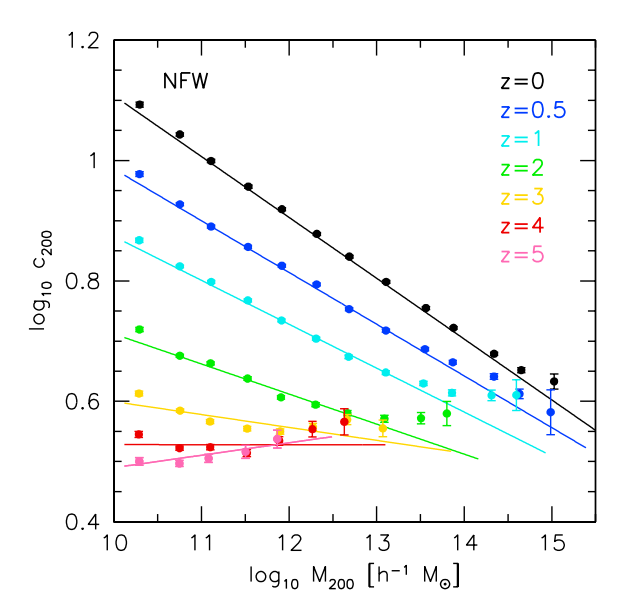
\includegraphics[width=10cm]{images/dutton.png}
\caption[Evolution of the concentration mass relation]{Evolution of the concentration mass relation, by \textcolor{blue}{Dutton \& Maccio} (\citeyear{Reference23}).}
\end{figure}

The surface mass density in the NFW profile (\textcolor{blue}{Wright \& Brainerd}, \citeyear{Reference4}) is given by:

\begin{equation}
\Sigma_{\text{NFW}}(x) = \left\lbrace
\begin{array}{lll}
\frac{2r_{s}\delta_{c}\rho_{c}}{\left(x^{2}-1\right)}\left[1-\frac{2}{\sqrt{1-x^{2}}}\arctanh\sqrt{\frac{1-x}{1+x}}\right] & (x<1)\\\\
\frac{2r_{s}\delta_{c}\rho_{c}}{3} & (x=1)\\\\
\frac{2r_{s}\delta_{c}\rho_{c}}{\left(x^{2}-1\right)}\left[1-\frac{2}{\sqrt{x^{2}-1}}\arctan\sqrt{\frac{x-1}{1+x}}\right] & (x>1)
\end{array}
\right.
\end{equation} 

so from the critical density:

\begin{equation}
\rho_{c}=\frac{3H^2(z)}{8\pi G}
\end{equation}

$H(z)=H_{0}(1+\Omega z)^{3/2}$

But we are more interested in the enclosed mass which can be done by integrating the surface mass density:

\begin{equation}
\text{M}(R)=\int_{0}^{R}2\pi R\Sigma(R)dR
\end{equation}

The radial dependence on the shear is:

\begin{equation}
\gamma_{\text{NFW}}(x) = \left\lbrace
\begin{array}{lll}
\frac{r_{s}\delta_{c}\rho_{c}}{\Sigma_c}g_{<}(x) & (x<1)\\\\
\frac{r_{s}\delta_{c}\rho_{c}}{\Sigma_c}\left[\frac{10}{3}+4 \ln \left(\frac{1}{2}\right)\right] & (x=1)\\\\
\frac{r_{s}\delta_{c}\rho_{c}}{\Sigma_c}g_{>}(x) & (x>1)
\end{array}
\right.
\end{equation} 

where: 

\begin{equation}
g_{<}(x)=\frac{8 \arctanh \sqrt{\frac{1-x}{1+x}}}{x^{2}\sqrt{1-x^{2}}}+\frac{4}{x^{2}} \ln \left(\frac{x}{2}\right)-\frac{2}{\left(x^{2}-1\right)}+\frac{4 \arctanh \sqrt{\frac{1-x}{1+x}}}{\left(x^{2}-1\right)\left(1-x^{2}\right)^{1/2}}
\end{equation}

\begin{equation}
g_{<}(x)=\frac{8 \arctan \sqrt{\frac{x-1}{1+x}}}{x^{2}\sqrt{x^{2}-1}}+\frac{4}{x^{2}}\ln \left(\frac{x}{2}\right)-\frac{2}{\left(x^{2}-1\right)}+\frac{4 \arctan \sqrt{\frac{x-1}{1+x}}}{\left(x^{2}-1\right){}^{3/2}}
\end{equation}  

For reference, Figure [2] shows strong systematic variation of the IMF in early-type galaxies as a function of their stellar mass-to-light ratio, producing differences up to a factor of three in mass by \textcolor{blue}{Cappellari et al.} (\citeyear{Reference19})

\begin{figure}[H]
\centering
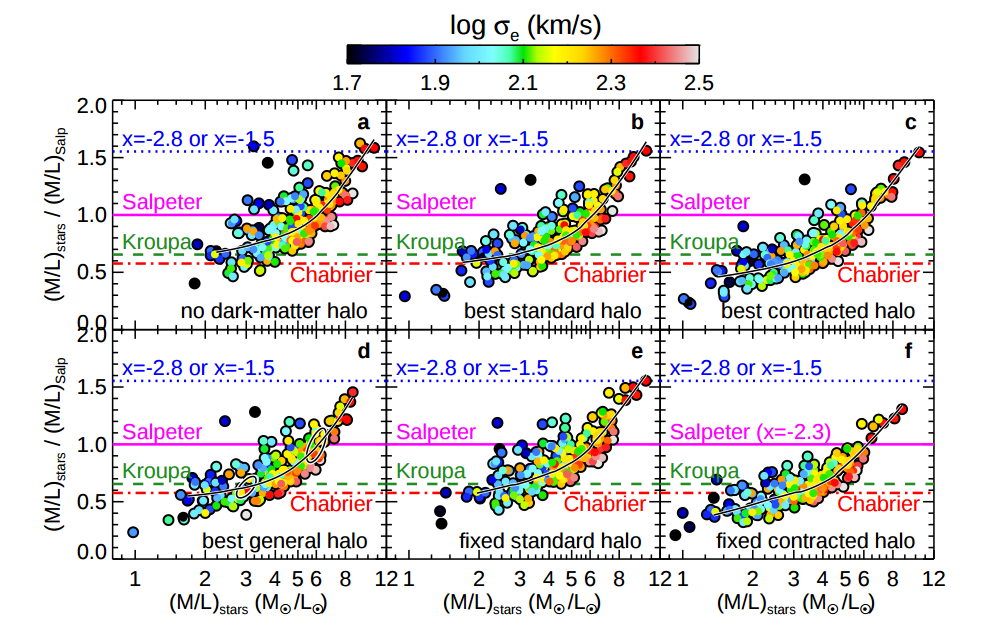
\includegraphics[width=12cm]{images/IMFs_paper.png}
\caption[The systematic variation of the IMF in early-type galaxies.]{The systematic variation of the IMF in early-type galaxies, \textcolor{blue}{Cappellari et al.} (\citeyear{Reference19}).}
\end{figure}
 
\end{appendices}